\documentclass[11pt]{beamer}

\usetheme{metropolis}

\usepackage{graphicx}
\usepackage{physics}
\usepackage{adjustbox}
\usepackage{caption}
\usepackage{chemformula}
\usepackage{quoting}
\usepackage[style=chem-angew,backend=bibtex]{biblatex}
\bibliography{references}
%
% Choose how your presentation looks.
%
% For more themes, color themes and font themes, see:
% http://deic.uab.es/~iblanes/beamer_gallery/index_by_theme.html
%
\mode<presentation>
{
  \usetheme{default}      % or try Darmstadt, Madrid, Warsaw, ...
  \usecolortheme{default} % or try albatross, beaver, crane, ...
  \usefonttheme{default}  % or try serif, structurebold, ...
  \setbeamertemplate{navigation symbols}{}
  \setbeamertemplate{caption}[numbered]
  \setbeamerfont{footnote}{size=\tiny}
} 

\usepackage[english]{babel}
\usepackage[utf8]{inputenc}
\graphicspath{{image/}}

\AtBeginSection[]{
\begin{frame}{Outline}
  \tableofcontents[currentsection]
\end{frame}
}

\title{Chapter 7: Electron Structure of the Atom}
\institute{Chemistry Department, Cypress College}
\date{October 24, 2022}

\begin{document}

\begin{frame}
  \titlepage
\end{frame}

\begin{frame}{Class Announcements}
  \textbf{Lab}
  \begin{itemize}
  \item Experiment 15 - Quantitative Prep of KCl
  \item Begin the water bath ASAP
  \item Reminder - Need $70\%$ of laborator points to pass
    the course
  \end{itemize}

  \textbf{Lecture}
  \begin{itemize}
  \item Ch 7 Bonus Lecture - Introduction to Quantum Chemistry
  \item Go over homework 7 (EC for students who present)
  \item Quiz and Homework assignment released Fri, Oct 14th at 3pm
  \item Exam 2 - Weds, Oct 26 at 2:55pm; 2 hours and 8 free response
    questions
  \end{itemize}
\end{frame}

\section{Review: Electromagnetic Radiation}

\begin{frame}{Revisit: Radiation Energy}
  \begin{center}
    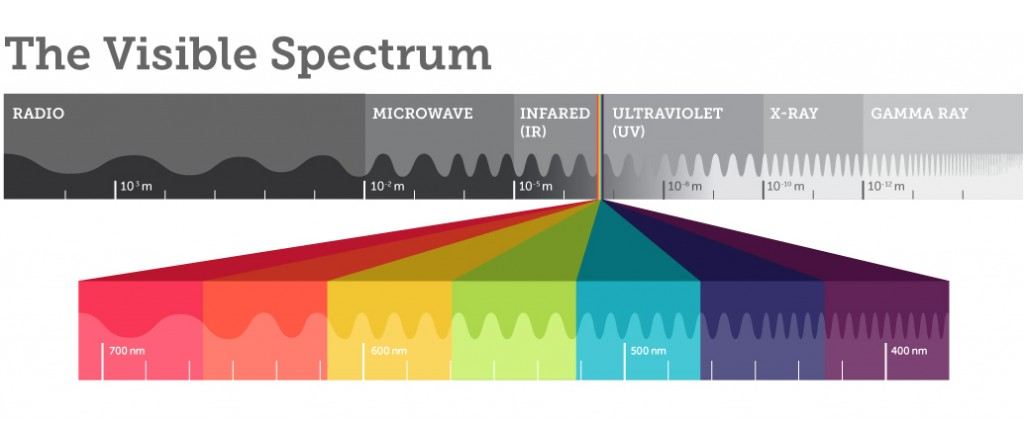
\includegraphics[width=0.85\linewidth]{visible_light}
  \end{center}
  \begin{equation}
    E = \frac{hc}{\lambda} = h\nu
    \label{eqn:photon}
  \end{equation}
  \begin{itemize}
  \item High frequency and larger wavelengths lead to higher radiation
    energy
  \item Energy are contained in packages known as photons; Eqn \ref{eqn:photon}
    computes the energy for 1 photon
  \end{itemize}
\end{frame}

\begin{frame}{Atomic Spectra}
  \centering
  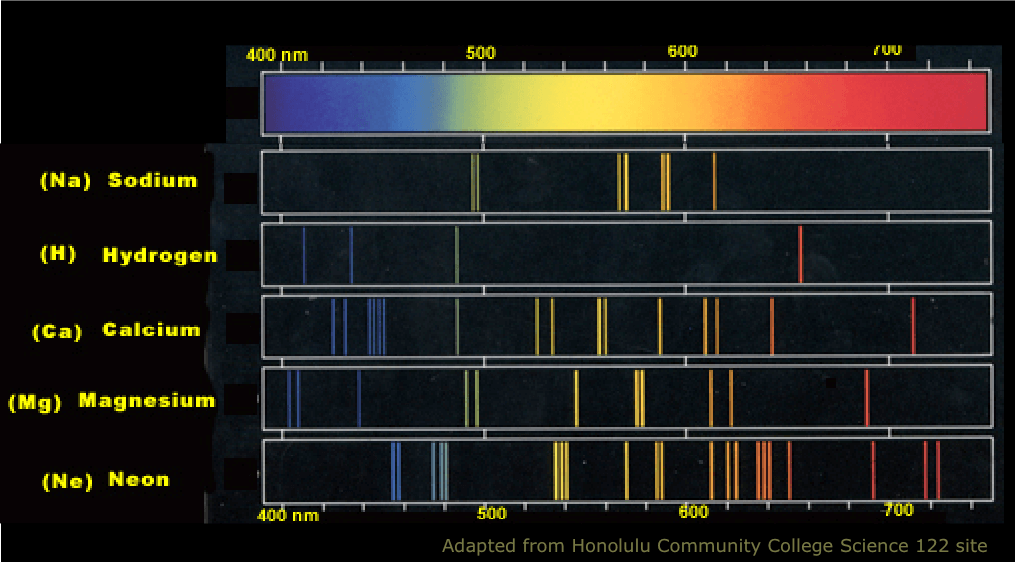
\includegraphics[width=0.85\linewidth]{cont_line}
  \begin{itemize}
  \item Continuous spectra is given at the top and
    discrete lines are emitted by atoms
  \item \textbf{Q:} Why are there discrete lines for
    the atomic spectra?
  \end{itemize}
\end{frame}

\begin{frame}{Bohr Model of the H Atom}
  \centering
  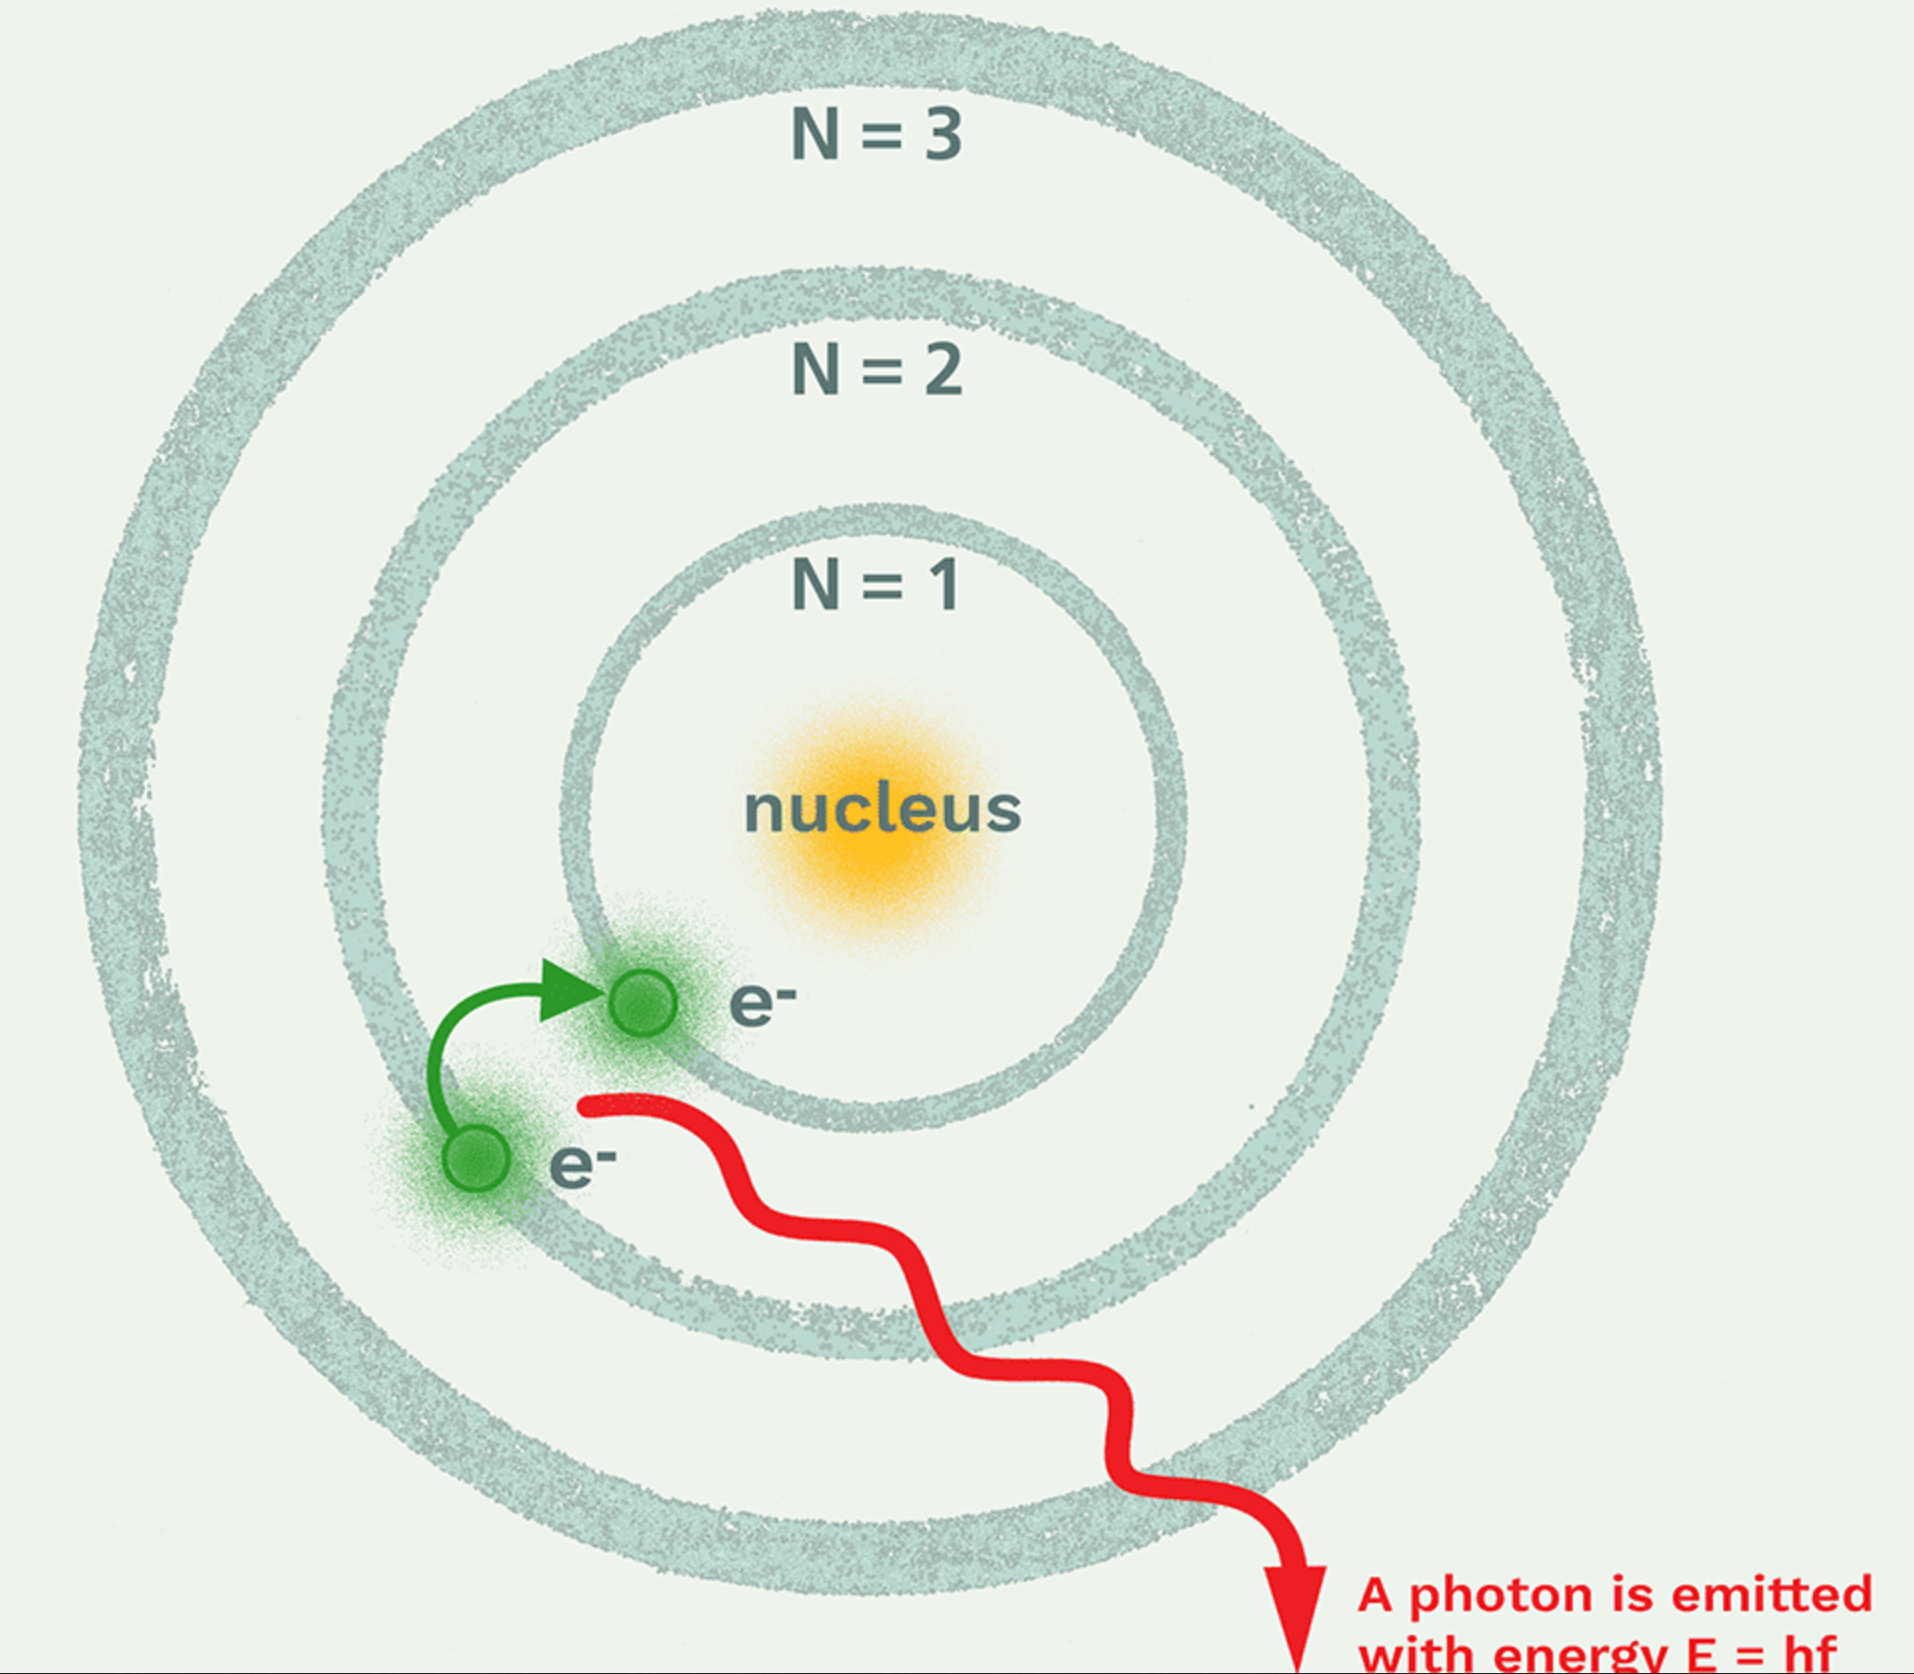
\includegraphics[width=0.55\linewidth]{bohr_model}
  \begin{align}
    \Delta E = & E_\text{final} - E_\text{initial}
  \end{align}
  Note: Keep in mind of sign conventions ($\Delta E > 0$ and
  $\Delta E < 0$)
\end{frame}

\begin{frame}{Bohr Model}
  \begin{itemize}
  \item Energy is quantized
  \item Electrons orbit the nucleus in orbits that have
    a set size and energy
  \item The energy of the orbit is related to its size; the
    lowest energy is found in the smallest orbit
  \item Radiation is absorbed or emitted when an electron
    moves from one orbit to another
  \end{itemize}
\end{frame}

\begin{frame}{Limitation of the Bohr Model}
  \begin{itemize}
  \item Violates the Heisenberg Uncertainty Principle
  \item Poor predictions regarding the spectra of larger
    atoms
  \item Does not predict the relative intensities of spectral
    lines
  \end{itemize}
\end{frame}

\begin{frame}{Example: H atom spectra}
  \begin{center}
    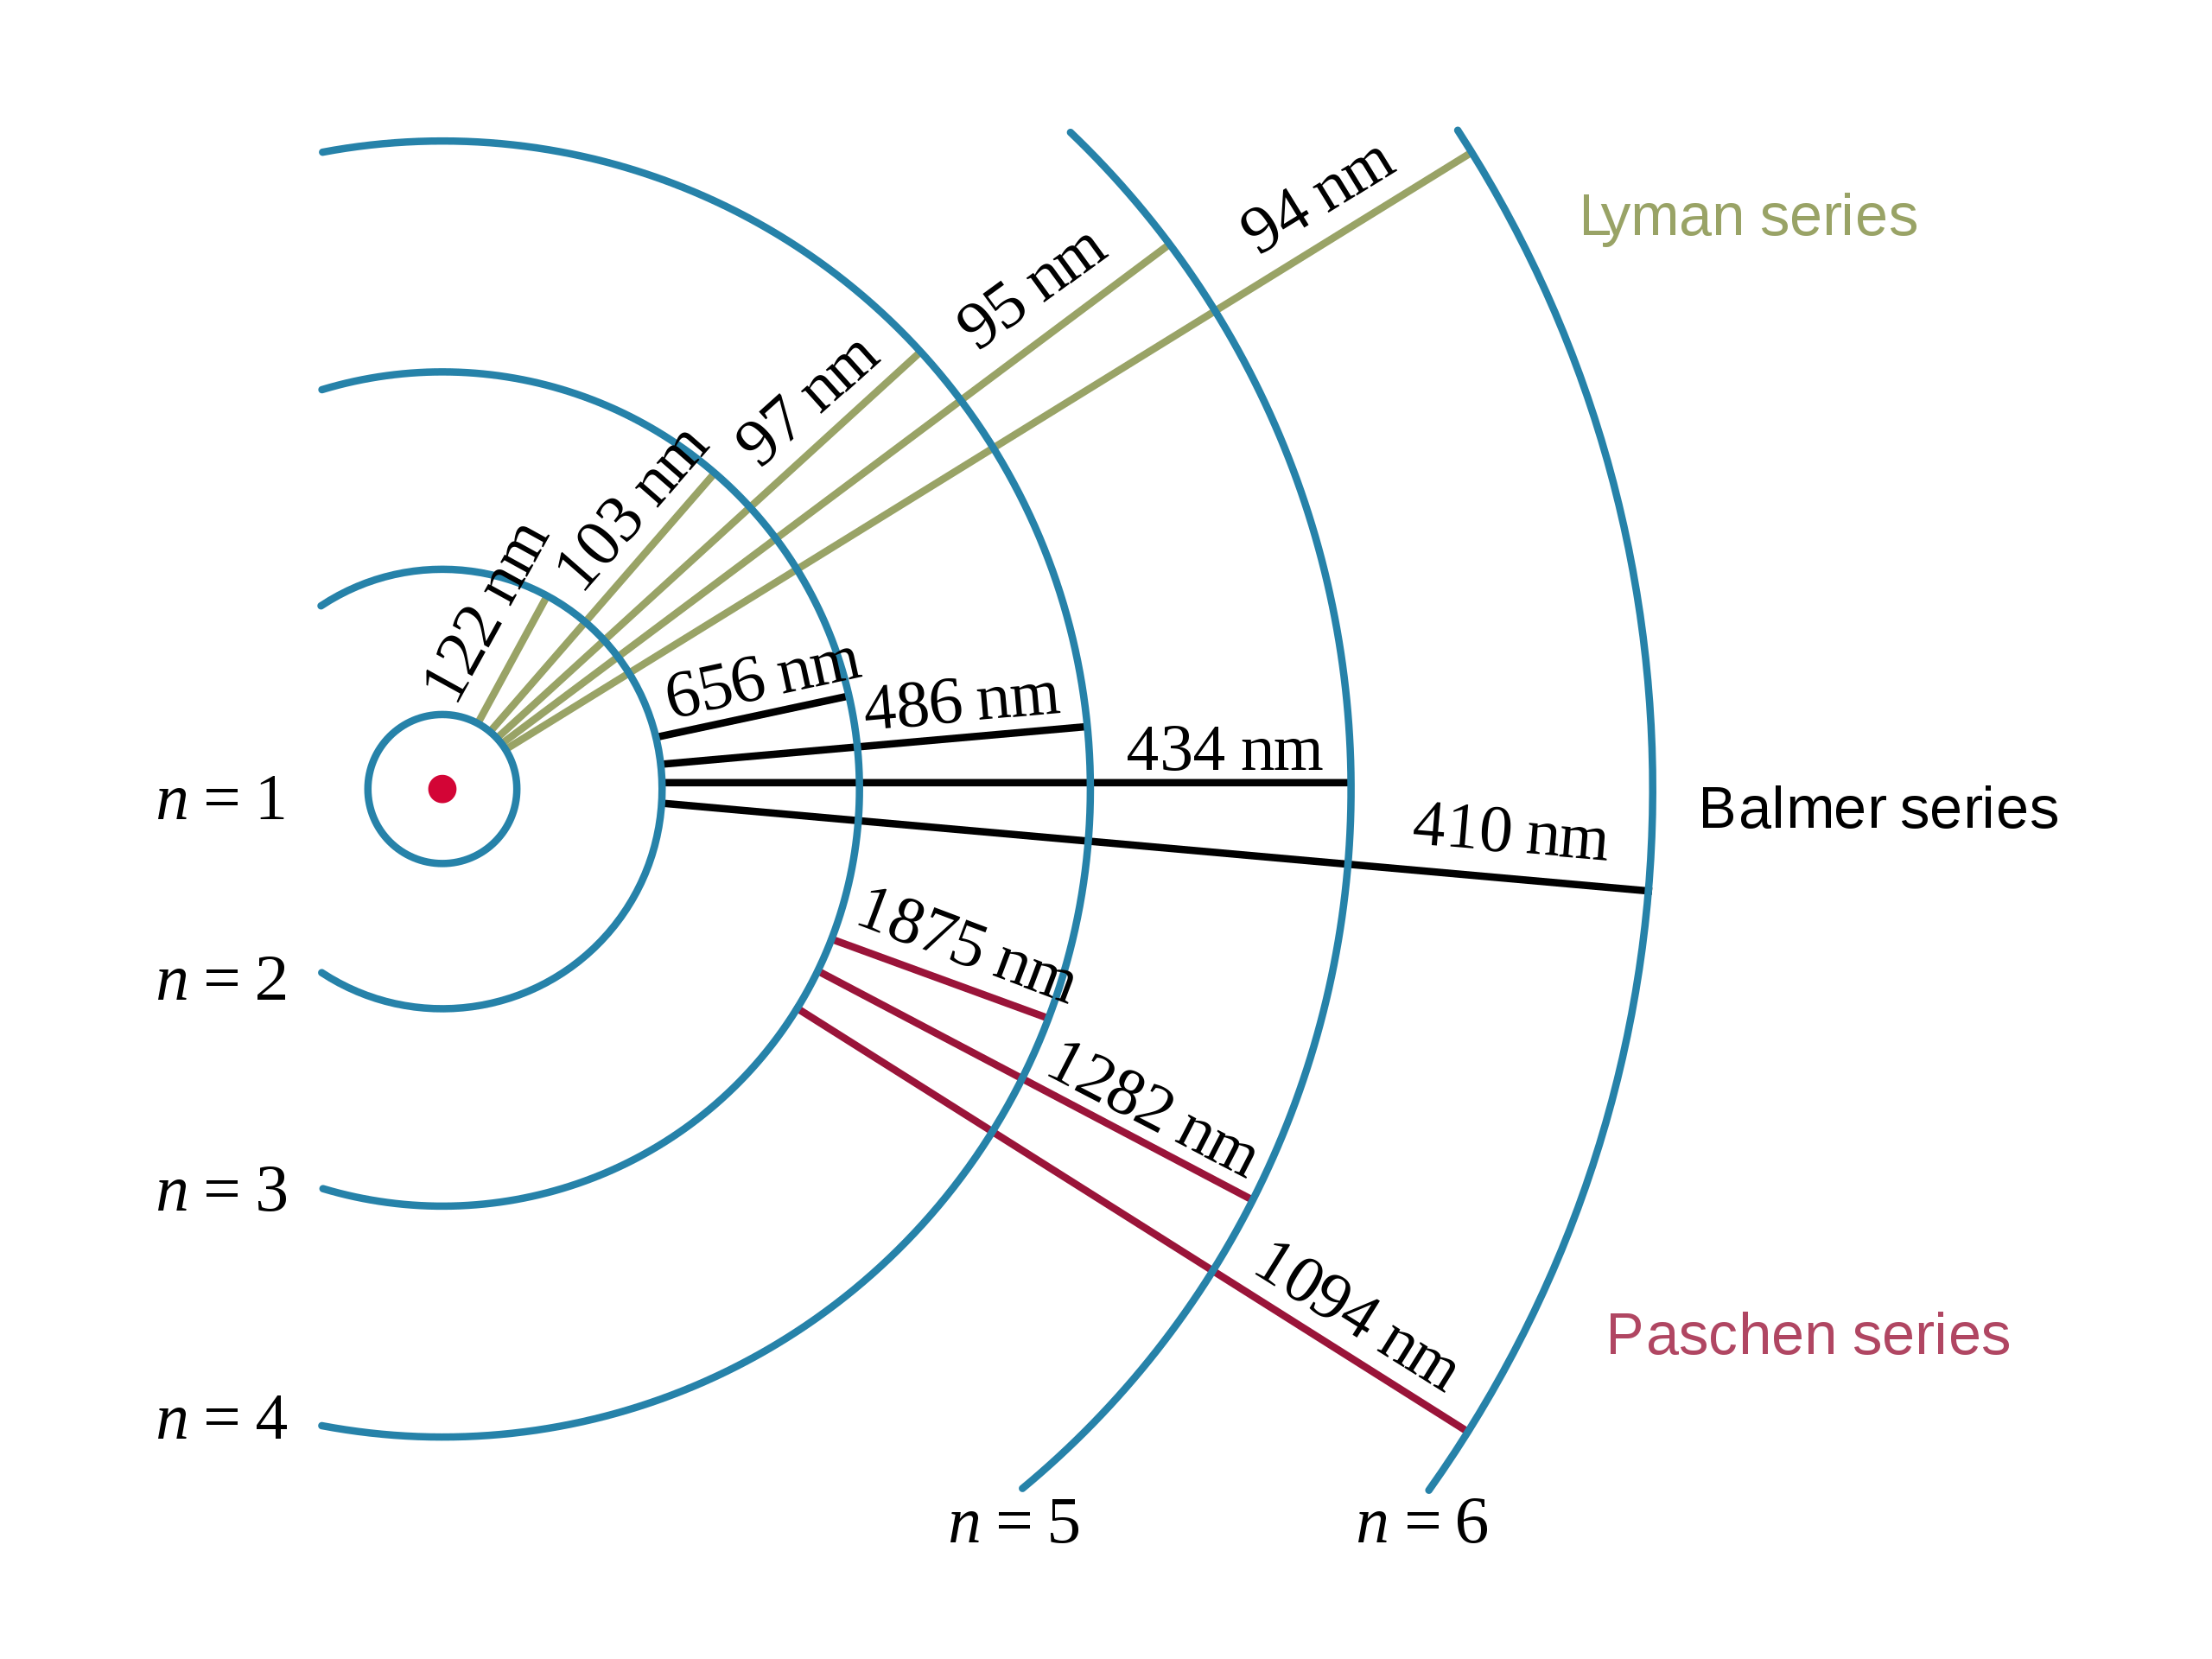
\includegraphics[scale=0.09]{h_spectra}
  \end{center}
\end{frame}

\section{Modern Model of the Atom}

\begin{frame}{Introduction to Quantum Chemistry}
  \textbf{Schr\"{o}dinger's Cat} - Thought Experiment
  \begin{center}
    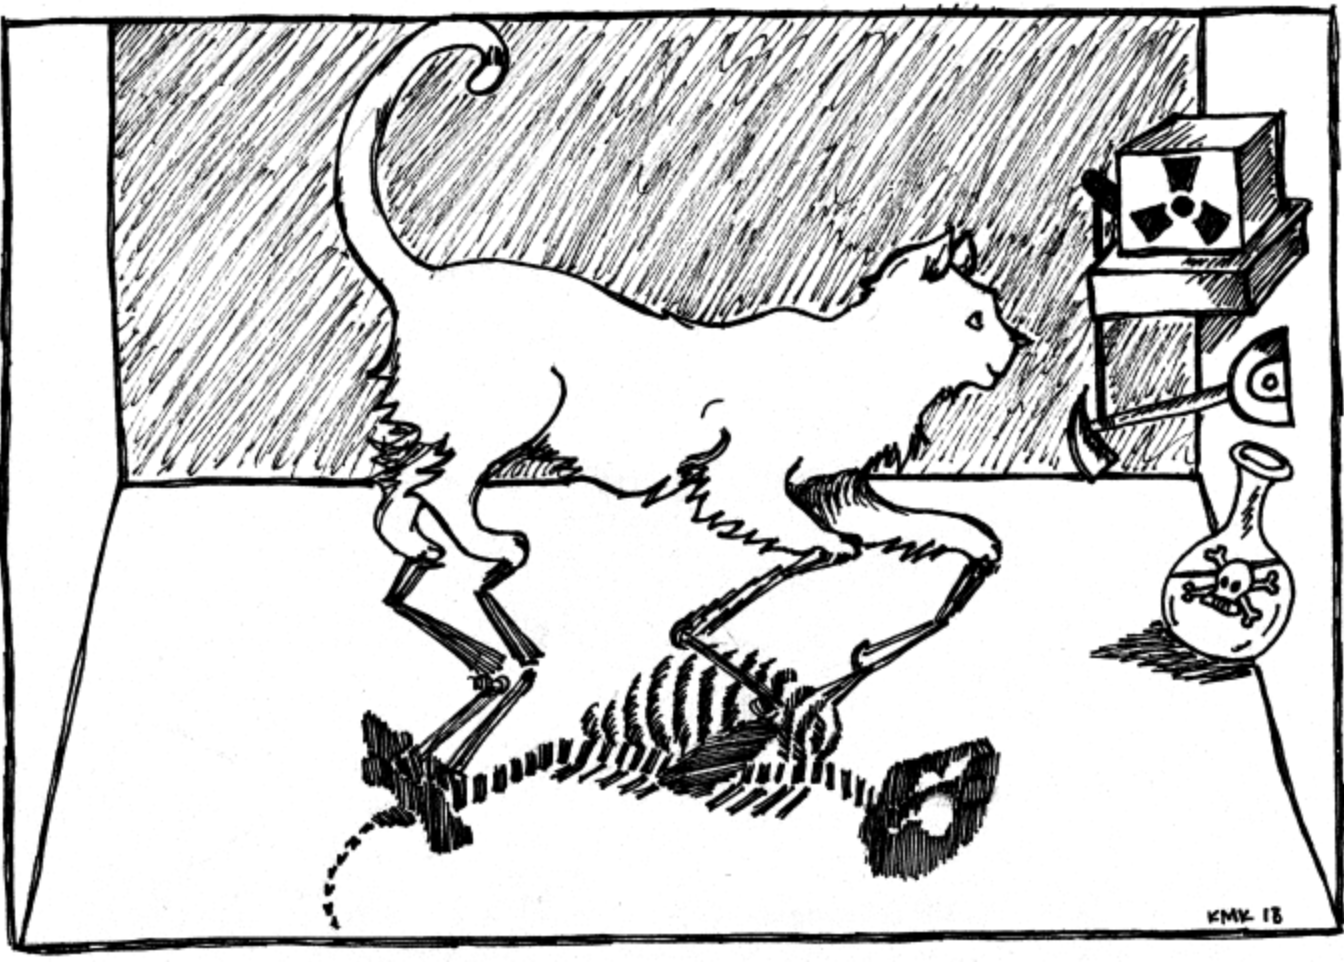
\includegraphics[width=0.65\linewidth]{schor_cat}
  \end{center}

  The world that we know is deterministic, however, dealing
  with electrons or small subatomic particles, we have to think
  of it in terms of probabilities
\end{frame}

\begin{frame}{The Wavefunction $\Psi$}
  \textbf{Schr\"{o}dinger's Equation}
  \begin{equation}
    \hat{H}\Psi = E\Psi
  \end{equation}
  where $\hat{H}$ is the Hamiltonian, $E$ is the energy,
  and $\Psi$ is the wavefunction
  \begin{itemize}
  \item Equation that explain everything about your system
  \item Chemical and physical properties can be determined
    from the $\Psi$
  \end{itemize}
\end{frame}

\begin{frame}{Properties of the $\Psi$}
  \begin{itemize}
  \item All measurable information about the particle is available
  \onslide<2->{\item $\Psi$ should be continuous and single-valued}
  \onslide<3->{\item Probability distribution in three dimensions is established
    using the $|\Psi|^2$}
  \onslide<4->{\item The probability of finding a particle if it exists is 1.}
  \end{itemize}
\end{frame}

\begin{frame}{Postulates of Quantum Mechanics}
  \begin{itemize}
  \item Everything about your system is describe by your $\Psi$ given
    the position $x$ and time $t$
  \onslide<2->{\item For every observable, there corresponds a Hermitian operator
    in quantum mechanics}
  \onslide<3->{\item In any measurement of the observable associated with operator
    $\hat{A}$, the only values that will ever be observed are the eigenvalues $a$,
    which satisfy the eigenvalue equation
    \begin{equation}
      \hat{A}\Psi = a\Psi
    \end{equation}
    }
  \end{itemize}
\end{frame}

\begin{frame}{Postulates of Quantum Mechanics}
  \begin{itemize}
  \item If a system is in a state described by a normalized wave function $\Psi$,
    then the average value of the observable corresponding to $\hat{A}$ is given by
    \begin{equation}
      \langle A \rangle = \int^\infty_{-\infty} d\tau \Psi^*\hat{A}\Psi
    \end{equation}
  \onslide<2->{\item Wavefunction is described by the Schr\"{o}dinger equation
    \begin{equation}
      \hat{H}\Psi = E\Psi
    \end{equation}
    }
  \onslide<3->{\item Total wavefunction must be antisymmetric with respect to the interchange of
    all coordinates of the electrons
    \begin{equation}
      \Psi(-x) = -\Psi(x)
    \end{equation}
    }
  \end{itemize}
\end{frame}

\begin{frame}{Atomic Orbitals}
  \centering
  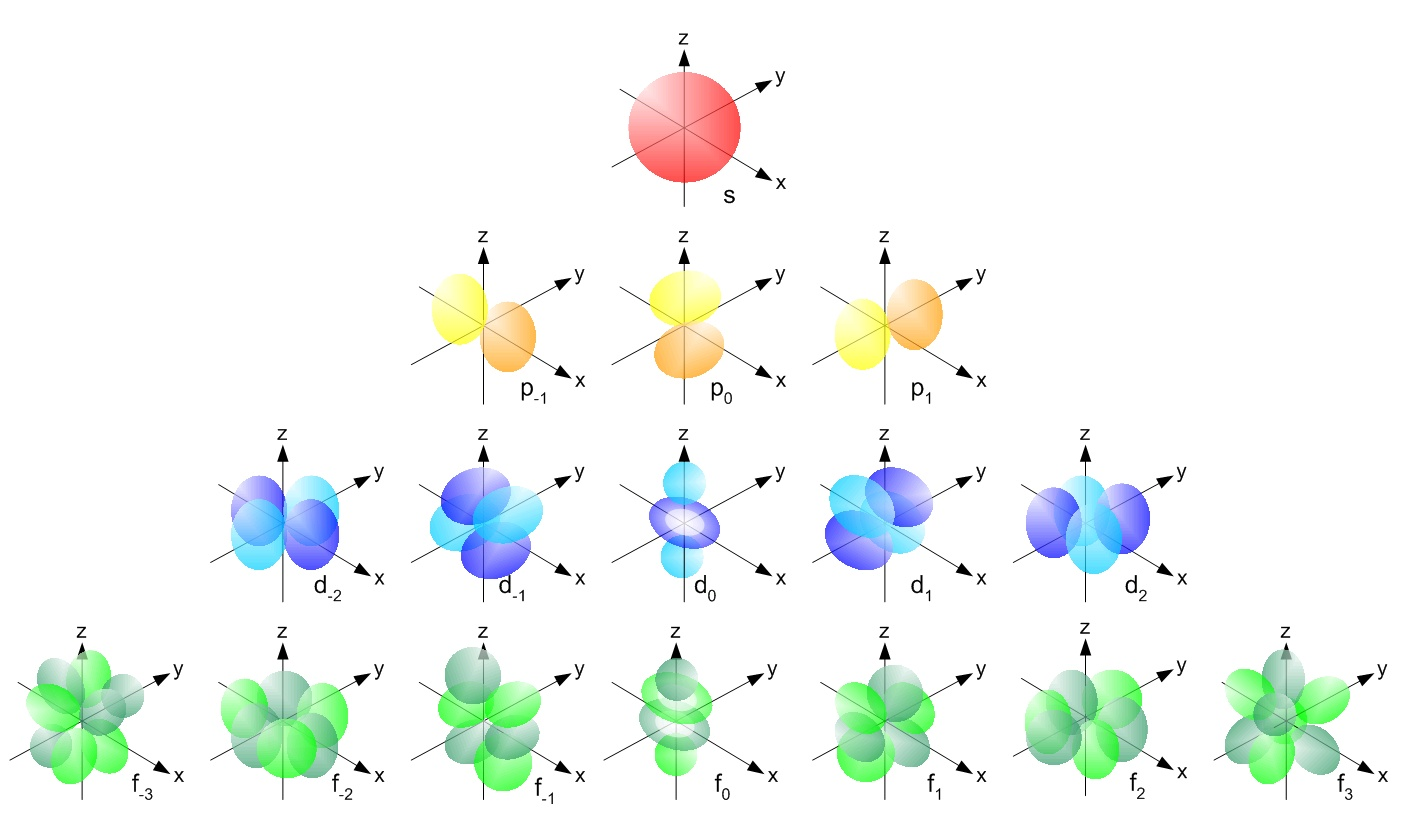
\includegraphics[width=\linewidth]{single_elect_orb}
\end{frame}

\end{document}
